\section{Graphics}
The graphics module is an abstract layer built on top of the HTML5 Canvas API. It abstracts away less used methods and implements higher level functionality such the ability to create view-ports and to draw points in various ways.

The API is built on the chaining principle; methods return the object on which they were invoked. This allows for very succinct way of drawing graphics:
\begin{verbatim}
  graphics.
    beginPath().
      moveTo(10, 10).
	  lineTo(20, 20).
    endPath().
    stroke('#00000');
\end{verbatim}
The graphics API has two basic types of methods, one to create shapes and the other to create paths. Shapes include the following methods: \code{beginViewport}, \code{closeViewport}, \code{beginPath}, \code{stroke}, \code{fill}, \code{rect}, \code{line}, points (i.e. \code{circle}, \code{triangle}, \code{cross}, \code{diamond}, etc.), and \code{text}. Paths include the following methods: \code{lineTo}, \code{moveTo}, \code{arcTo}, \code{bezierCurveTo}, \code{quadraticCurveTo}, \code{closePath}, and \code{endPath}. Shapes can be considered ready-made instances of paths (although the implementation might differ) and they define a higher level interface to drawing complex paths.

The graphics object does not expose path methods, instead the \code{beginPath} method returns a set of functions that can create paths. Once the user is creating a path there is no way---other than by calling either the \code{closePath} or \code{endPath} methods (which returns the shapes set of methods)---to return to the shape group. This enforces the correct creation of paths and shapes (i.e. the API ensures that only valid method call combinations are made.)

\subsection{Custom view-ports}
The chart library implements its own transformation stack instead of using the one provided by the HTML5 Canvas API. The reason for this is to have complete control over how lines are drawn. This can only be achieved by not using the built-in transformation stack. An example of one of the problems is that line width is not implemented consistently across browsers and transformation states. Some browsers will use the line width associated with the transformation matrix when the path was created, while others will use the line width associated with the transformation matrix when the path was stroked. The following HTML5 Canvas example demonstrates this problem.
\begin{verbatim}
  ctx.lineWidth = 2;
  ctx.save();
  ctx.scale(1.5, 1.5);
  ctx.lineTo(10, 10);
  ctx.store();
  ctx.stroke();
\end{verbatim}
Some implementations will stroke the path with a line width of 2, while others will use a line width of 3 (2 scaled by 1.5). Unfortunately---and unlike other graphics APIs, such as OpenGL \cite{shreiner05}---the HTML5 Canvas element does not specify a stack for rendering properties such as line width. To overcome this problem, it was necessary to implement a custom transformation stack. The graphics module supports this through two methods: \code{beginViewport} and \code{closeViewport}. Instead of offering more general \code{scale} and \code{translate} methods, these methods deal with the concept of a viewport; a two dimensional area, with its own custom coordinate system. The \code{beginViewport} method takes four required parameters (\code{x}, \code{y}, \code{width}, and \code{height}) and three optional ones (horizontal interval, vertical interval, and polar.) When the horizontal and vertical intervals are specified, all drawing between the \code{beginViewport} and \code{closeViewport} method calls are performed in those intervals. This simplifies drawing data points by removing the need for transforming the data into the charts' view port; data can simply be plotted to the screen without transformation. Viewports can also be nested without problems.

The last optional parameter is polar, which, when turned on, transforms the coordinates to all drawing methods from polar to Cartesian. This makes it possible to also transparently plot polar data.

\subsection{Crisp line drawing}
Although it has support for some vector operations, the HTML5 Canvas element is not a vector based API, it basically draws bitmaps. As such, it becomes a necessity to manually ensure that lines are drawn on screen pixels instead of on pixel boundaries resulting in an approximation\cite{shepherd08} (blurred lines.) Figure \ref{crisp} shows two lines on a pixel grid. The red lines indicate the vector representation of the lines, and the blue filled area the actual screen pixels. The first line is drawn on pixel boundaries and thus results in an approximation, the right line on the other hand is drawn at exactly the center of a pixel and thus results in a crisp line drawing.

\begin{figure}[h!]
\centering
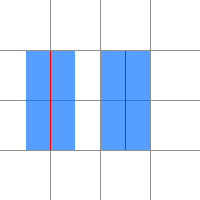
\includegraphics[width=.35\linewidth]{crisp}
\caption{Approximated line and crisp drawn line}
\label{crisp}
\end{figure}

The graphics module internally ensures that all lines and rectangles are drawn on screen pixels and never on the boundaries. As this "rounding" to screen pixels is done consistently, the resulting image is not affected, other than being slightly moved up or down (depending on the implementation of the rounding.)

\subsection{Fonts/Text support}
Unfortunately font and text drawing support in the HTML5 Canvas element is not well developed at the moment. Only Firefox 3.1 and Safari implement a standardized text drawing API. Firefox also offers its own alternative text drawing API. Both Internet Explorer and Opera have no support for drawing text on a HTML5 Canvas (Internet Explorer does in fact not support the Canvas element at all.) The standardized text API is also severely lacking in functionality. For example, it is possible to retrieve the width of a string in pixels, but not the height. Text is not treated as a set of paths, but drawn directly on the canvas through two separate \code{fillText} and \code{strokeText} functions. Strangely enough, the alternative Firefox text API does offer support for treating text as paths, and offers the ability to then stroke or fill those paths. Direct drawing versus paths is a not a big issue in the development of this chart library, but the font metrics problems are a big issue when aligning labels, legends, and titles.

In order to overcome these problems the chart library uses the HTML DOM to insert the a properly stylized string into an offscreen location in the surrounding HTML page and retrieve correct font metrics that way. In future versions of the library it might be possible to replace this with a better standardized and implemented HTML5 Canvas text API. Alternatively, it would be possible to overlay absolutely positioned HTML elements on top of the HTML canvas \cite{steele06}, use a bitmap font, or use one of the available path based fonts \cite{studt07, effenberger08, greenpoint08}.

\subsection{Browser support}
Firefox, Opera and Safari all support various subsets of the HTML5 Canvas tag. Fortunately there is a common subset of functionality that is sufficient for use in the chart library (apart from a text API.) Unfortunately, the only browser that does not support HTML5 Canvas is also the browser with the largest market share: Internet Explorer. Fortunately there are JavaScript implementations available that provide a HTML5 Canvas API for Internet Explorer and convert the API calls into VML elements \cite{google08}. By using one of these JavaScript implementations, the chart library supports all major browsers.
